\documentclass[compress,red]{beamer}
\usepackage[utf8]{inputenc}
\usepackage{ucs}
\usepackage{amsmath}
\usepackage{amsfonts}
\usepackage{amssymb}
\usepackage[russian]{babel}
\usepackage{graphicx}
\usepackage{wrapfig}

\usepackage{tikz}
\usepackage{verbatim}

\usepackage{color}
\usepackage{xcolor}
\usepackage{listings}

\usepackage{caption}

\lstset{
language=ruby,
extendedchars=\true,
inputencoding=utf8x,
commentstyle=\itshape,
stringstyle=\bf,
belowcaptionskip=5pt }


\DeclareCaptionFont{white}{\color{white}}
\DeclareCaptionFormat{listing}{\colorbox{gray}{\parbox{\textwidth}{#1#2#3}}}
\captionsetup[lstlisting]{format=listing,labelfont=white,textfont=white}

\usetikzlibrary{calc,trees,positioning,arrows,chains,shapes.geometric,%
    decorations.pathreplacing,decorations.pathmorphing,shapes,%
    matrix,shapes.symbols}

\tikzset{
>=stealth',
  punktchain/.style={
    rectangle, 
    rounded corners, 
    % fill=black!10,
    draw=black, very thick,
    text width=10em, 
    minimum height=3em, 
    text centered, 
    on chain},
  line/.style={draw, thick, <-},
  element/.style={
    tape,
    top color=white,
    bottom color=blue!50!black!60!,
    minimum width=8em,
    draw=blue!40!black!90, very thick,
    text width=10em, 
    minimum height=1.5em, 
    text centered, 
    on chain},
  every join/.style={->, thick,shorten <=1pt},
  decoration={brace},
  tuborg/.style={decorate},
  tubnode/.style={midway, right=2pt},
}

\mode<presentation>

\usetheme{Warsaw}

\definecolor{Red}{rgb}{1,0,0}
\definecolor{Blue}{rgb}{0,0,1}
\definecolor{Green}{rgb}{0,1,0}
\definecolor{magenta}{rgb}{1,0,.6}
\definecolor{lightblue}{rgb}{0,.5,1}
\definecolor{lightpurple}{rgb}{.6,.4,1}
\definecolor{gold}{rgb}{.6,.5,0}
\definecolor{orange}{rgb}{1,0.4,0}
\definecolor{hotpink}{rgb}{1,0,0.5}
\definecolor{newcolor2}{rgb}{.5,.3,.5}
\definecolor{newcolor}{rgb}{0,.3,1}
\definecolor{newcolor3}{rgb}{1,0,.35}
\definecolor{darkgreen1}{rgb}{0, .35, 0}
\definecolor{darkgreen}{rgb}{0, .6, 0}
\definecolor{darkred}{rgb}{.75,0,0}

\xdefinecolor{olive}{cmyk}{0.64,0,0.95,0.4}
\xdefinecolor{purpleish}{cmyk}{0.75,0.75,0,0}

\useoutertheme[subsection=false]{smoothbars}

\title{Кодирование}
\author{Информатика \\ 8 класс}

%\usecolortheme{dolphin}


\begin{document}
%%титульная страница
\maketitle
%% основные моменты

\section{Введение}
\subsection{Раз}
\begin{frame}
  \frametitle{Информация}
  \begin{itemize}
    \item Информация окружает человека повсюду.
    \item Живущий в информационном обществе индивид постоянно занимается поиском, обработкой, хранением и анализом информации.
    \item Информация, доводимая до общества, должна быть \emph{достоверной} и \emph{актуальной}, в противном случае недостоверная информация вводит членов общества в заблуждение.
    \item Перед наукой стоит задача в поиске \emph{полной} и \emph{точной информации}.
  \end{itemize}
\end{frame}

\section{Классификация}
\subsection{Классификация}
\begin{frame}
  \begin{center}
    \Huge{Классификация информации}
  \end{center}
\end{frame}

\subsection{Визуальная}
\begin{frame}[fragile]
  \frametitle{Визуальная}
  \centerline{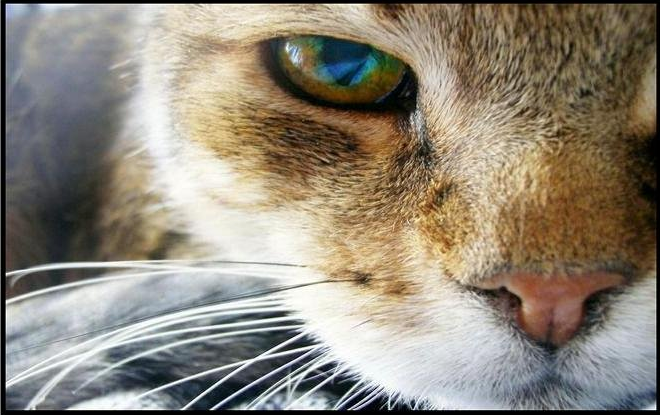
\includegraphics[width=0.9\textwidth]{images/cat_eye.png}}
\end{frame}

\subsection{Тактильная}
\begin{frame}[fragile]
  \frametitle{Тактильная}
  \centerline{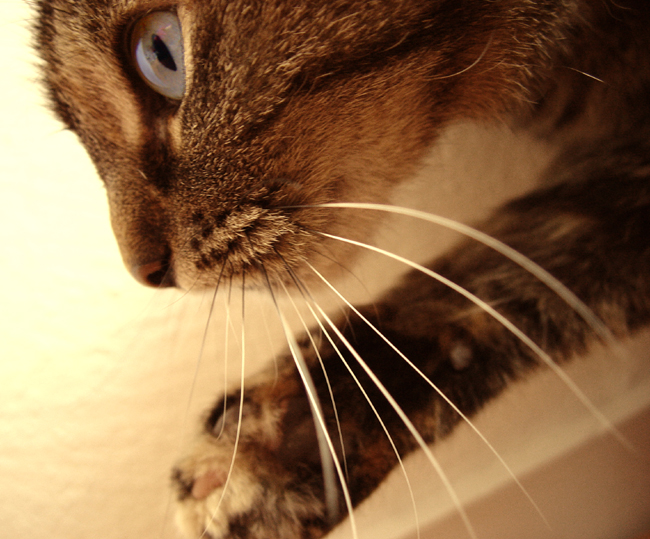
\includegraphics[width=0.7\textwidth]{images/cat_whiskers.jpeg}}
\end{frame}

\subsection{Органолентическая}
\begin{frame}[fragile]
  \frametitle{Органолентическая (запах и вкус)}
  \centerline{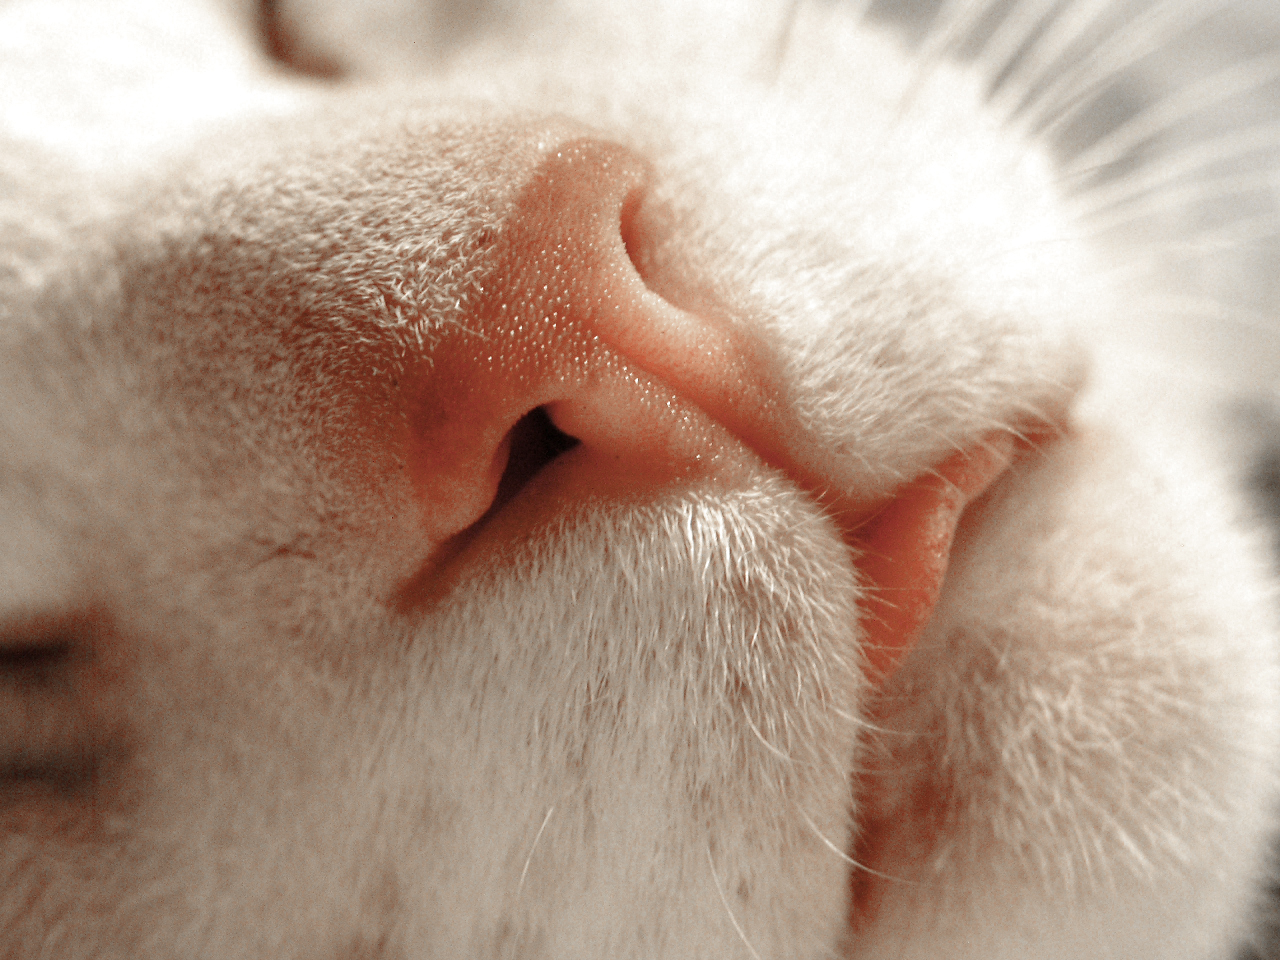
\includegraphics[width=0.8\textwidth]{images/cat_nail.jpeg}}
\end{frame}

\subsection{Аудиальная}
\begin{frame}[fragile]
  \frametitle{Аудиальная}
  \centerline{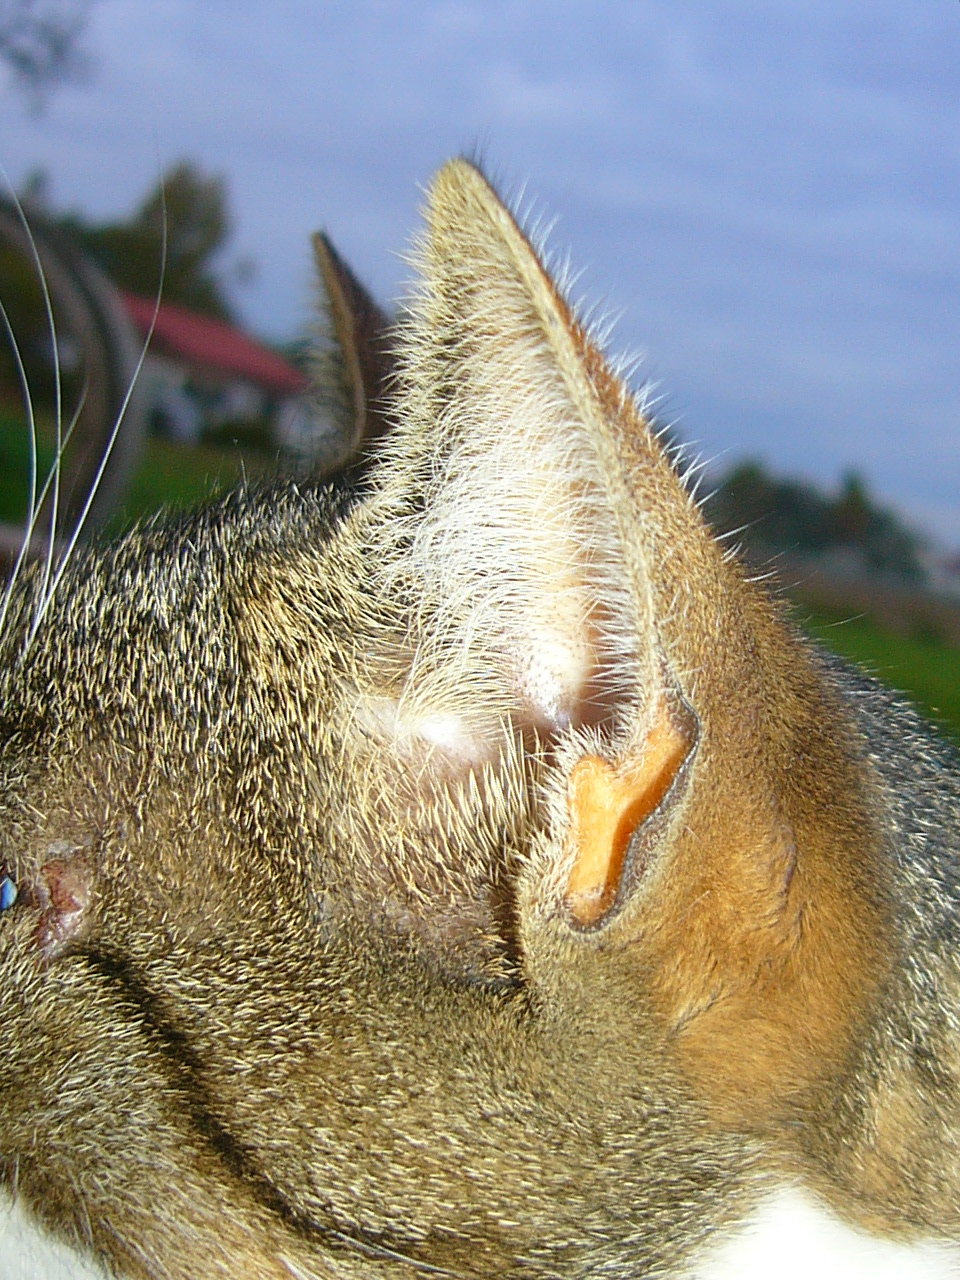
\includegraphics[width=0.5\textwidth]{images/cat_ear.jpeg}}
\end{frame}

\subsection{Машиинно-выдаваемая}
\begin{frame}[fragile]
  \frametitle{Машинно-выдаваемая и воспринимаемая}
  \centerline{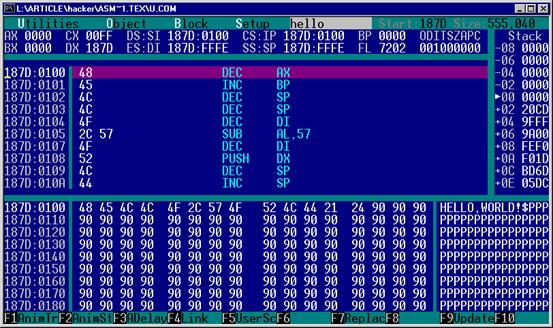
\includegraphics[width=0.9\textwidth]{images/computer_info.jpeg}}
\end{frame}

\subsection{Передача информации}
\begin{frame}[fragile]
  \frametitle{Передача информации}
  
  \begin{figure}
  \centering
  \begin{tikzpicture}[node distance=1cm, auto]  
  \tikzset{
      action/.style={rectangle,draw=black, top color=white, bottom color=yellow!50,very thick, inner sep=0.25em, minimum size=0.6em, text centered},
      input/.style={ellipse,draw=black, top color=white, bottom color=yellow!50,very thick, inner sep=0.25em, minimum size=0.6em, text centered},
      condition/.style={diamond,draw=black, top color=white, bottom color=yellow!50,very thick, inner sep=0.25em, minimum size=0.6em, text centered},
      myarrow/.style={draw},
  }
  \node[action]  (item1) {Источник};
  \node[action, right=of item1]  (item2) {КУ};
  \node[action, right=of item2,xshift=2cm]  (item3) {ДУ};
  \node[action, right=of item3]  (item4) {Приёмник};
  \path[line] (item2) -- node [near end] {} (item1);        
  \path[line] (item3) -- node [near end,xshift=0.6cm] {канал связи} (item2);        
  \path[line] (item4) -- node [near end] {} (item3);        

  \end{tikzpicture} 
  \end{figure}
  
  \begin{itemize}
    \item КУ --- кодирующее устройство,
    \item ДУ --- декодирующее устройство.
  \end{itemize}
  
\end{frame}

\section{Алфавит}

\subsection{Алфавит}
\begin{frame}
  \begin{center}
    \Huge{Алфавит}
  \end{center}
\end{frame}

\subsection{Алфавит}
\begin{frame}
  \begin{center}
    \Huge{Алфавит}
  \end{center}
  \begin{center}
    \Large{Непересекающийся набор символов}
  \end{center}
\end{frame}

\subsection{Старославянский алфавит}
\begin{frame}[fragile]
  \frametitle{Старославянский алфавит}
  \centerline{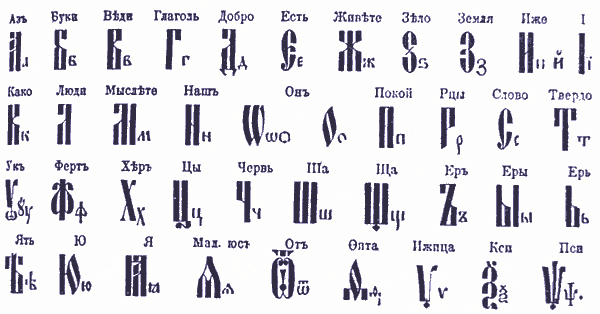
\includegraphics[width=0.9\textwidth]{images/alphabet_old_slavic.png}}
\end{frame}

\subsection{Греческий алфавит}
\begin{frame}[fragile]
  \frametitle{Греческий алфавит}
  \centerline{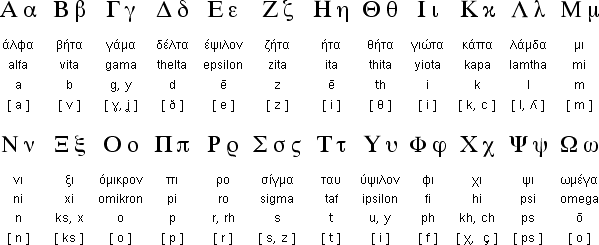
\includegraphics[width=0.9\textwidth]{images/alphabet_greek.png}}
\end{frame}

\subsection{Произвольный}
\begin{frame}[fragile]
  \frametitle{Произвольный алфавит}
  \begin{center}
    \Huge{:)\ \ :(\ \ :|\ \ :D\ \ :P}\newline\newline
    \Large{Алфавит может состоять из любых символов!}
  \end{center}
\end{frame}

\subsection{Мощность алфавита}
\begin{frame}[fragile]
  \frametitle{Мощность алфавита}
  \begin{itemize}
    \item Наборы символов из алфавита называются \textbf{словами}.
    \item Пример слов: \emph{мама} (русский алфавит), $\mu \alpha \mu \alpha$ (греческий), :):(:):) (произвольный).
    \item \emph{Мощность алфавита} --- количество символов в алфавите.
    \item Мощность русского алфавита --- 33 символа.
    \item Мощность английского алфавита --- 26 символов.
  \end{itemize}
\end{frame}

\section{Единицы измерения информации}
\subsection{Единицы измерения информации}
\begin{frame}[fragile]
  \frametitle{Единицы измерения информации}
  \begin{center}
    \Huge{Для измерения информации есть специальные единицы}.\newline
  \end{center}
\end{frame}

\subsection{Единицы}
\begin{frame}[fragile]
  \frametitle{Единицы измерения}
  \begin{table}
    \begin{center}
      \begin{tabular}{lll}
        \hline
        Величина & Перевод  & Байты \\
        \hline
        \onslide<2-6>{
        1 \ байт & 8 бит & $2^3$ бит \\
        \hline
        }
        \onslide<3-6>{
        1 Кбайт & 1024 байта & $2^{10}$ байт \\
        \hline 
        }
        \onslide<4-6>{
        1 Мбайт & 1024 Кбайт & $2^{20}$ байт \\
        \hline
        }
        \onslide<5-6>{
        1 Гбайт & 1024 Мбайт & $2^{30}$ байт \\
        \hline
        }
        \onslide<6>{
        1 Тбайт & 1024 Гбайт & $2^{40}$ байт \\
        \hline
        }
      \end{tabular}
    \end{center}
  \end{table}
\end{frame}

\subsection{Бит}
\begin{frame}
  \begin{center}
    \Huge{Бит --- минимальная единица информации}
  \end{center}
\end{frame}

\subsection{Бит 2}
\begin{frame}[fragile]
  \frametitle{Бит}
  \begin{itemize}
    \item Кодирование двух равновероятных состояний системы --- один бит.
    \item Например, количество информации, получаемое от ответа ``Да'' или ``Нет'' на какой-либо вопрос, равно 1~биту.
    \item Результат бросания монетки (орёл, решка) также содержит 1~бит информации.
    \item Для кодирования большего числа состояний нужно больше бит.
    \item Если у нас есть 2 бита, то мы можем закодировать 4 символа: для каждого из двух состояний первого бита есть два состояния второго бита.
    \item А если 3? Для каждого из 2 состояний первого бита есть два состояния второго. Для каждой из 4 пар первых двух бит есть две комбинации 3-го. Итого: $4*2 = 8$ символов.
  \end{itemize}
\end{frame}

\subsection{Количество символов}
\begin{frame}[fragile]
  \frametitle{Количество символов}
  \begin{table}
    \begin{center}
      \begin{tabular}{ccc}
      \hline
      Бит & Комбинаций  & Число \\
      \hline
      1 & $2^1$  & 2 \\
      \hline
      2 & $2^2$  & 4 \\
      \hline
      3 & $2^3$  & 8 \\
      \hline
      4 & $2^4$  & 16 \\
      \hline
      5 & $2^5$  & 32 \\
      \hline
      6 & $2^6$  & 64 \\
      \hline
      7 & $2^7$  & 128 \\
      \hline
      8 & $2^8$  & 256 \\
      \hline
      9 & $2^9$  & 512 \\
      \hline
      10 & $2^{10}$  & 1024 \\
      \hline
      \end{tabular}
    \end{center}
  \end{table}
\end{frame}

\subsection{Русский алфавит}
\begin{frame}[fragile]
  \frametitle{Русский алфавит}
  \begin{itemize}
    \item Рассмотрим, сколько бит будет занимать один символ русского алфавита.
    \item В русском алфавите --- 33 символа.
    \item Посмотрим в таблицу, сколько бит нам хватит. 5 бит не хватает, так как 5 бит кодирует только 32 символа, а нам надо 33. Значит, берём 6 бит. Они кодируют 64 символа, поэтому этого хватит даже с лихвой.
    \item Ответ: 1 символ русского алфавита занимает 6 бит.
  \end{itemize}
\end{frame}

\subsection{Задачи 1}
\begin{frame}[fragile]
  \frametitle{Задачи}
  \begin{itemize}
    \item Сколько бит занимает один символ английского алфавита?
    \item Сколько бит занимает один символ алфавита, состоящего из цифр?
    \item Сколько бит будет занимать слово ``мама'' в русском алфавите? А предложение ``There is no spoon'' в английском алфавите?
  \end{itemize}
\end{frame}

\subsection{Решение задачи 1}
\begin{frame}[fragile]
  \frametitle{Решение}
  \begin{itemize}
    \item В английском алфавите --- 26 символов (27 с учётом пробела). Для кодирования одного из них достаточно 5 бит (которые дают аж 32 символа, а у нас и того меньше. 4 не подойдёт, так как 4 бита кодируют только 16 комбинаций).
    \item Итого, 1 символ кодируется 5 битами.
    \item Посчитаем (с учётом пробелов) количество символов в предложении ``There is no spoon'': 17 символов.
    \item Составляем пропорцию: 1 символ --- 5 бит, 17 символов --- $x$.
    \item $x = 5\cdot 17 = 85$ бит.
  \end{itemize}
\end{frame}

\subsection{Перевод из бит в байты}
\begin{frame}[fragile]
  \frametitle{Перевод единиц измерения}
  \begin{itemize}
    \item \textbf{Задача}. У Васи имеется имеется доступ к Интернету со скоростью скачивания $2^{25}$~бит/с. Сколько он сможет скачать Мбайт за 10 секунд?
    \item \textbf{Решение}. Прежде всего, переведём бит/с в Мбайт/с. Для этого воспользуемся таблицей перевода: 1~Мбайт~=~$2^{23}$~бит.
    \item $\cfrac{2^{25}}{2^{23}} = 2^{25-23} = 2^2 = 4$ Мбайта.
    \item Итого, скорость Васи составляет 4 Мбайт/с.
    \item Значит, за 10с Вася скачает $4\cdot 10 = 40$ Мбайт информации.
    \item \textbf{Ответ:} 40 Мбайт.
  \end{itemize}
\end{frame}

\subsection{Задачи 2}
\begin{frame}[fragile]
  \frametitle{Задачи}
  \begin{itemize}
    \item У Пети имеется доступ к Интернету со скоростью $2^{28}$ бит/с. Сколько информации он скачает за 5 секунд?
    \item Вася хочет скачать фильм объёмом 4 Гбайта. Скорость соединения Васи с Интернетом составляет $2^{28}$ бит/с. Посчитайте, сколько времени потребуется Васе, чтобы скачать фильм.
    \item Маша скачивает программу из Интернета, которая занимает 128 Мбайт. Скорость соединения Маши с Интернетом составляет $2^8$ Кбайт/с. Сколько времени потребуется Маше, чтобы скачать всю программу.
  \end{itemize}
\end{frame}

\subsection{Решение задач 2}
\begin{frame}[fragile]
  \frametitle{Решение}
  \begin{itemize}
    \item Решим задачу с Машей.
    \item Переведём размер программы и скорость Интернета Маши в биты для простого сравнения.
    \item Программа: $128$ Мбайт = $128\cdot 2^{23}$ бит.
    \item Скорость: $2^8$~Кбайт/с $=$ $2^8\cdot 2^{13}$~бит/с $=$ $2^{21}$~бит/с.
    \item Разделим: $\cfrac{128\cdot 2^{23}}{2^{21}} = 128\cdot 2^{23-21} = 128\cdot 2^2 = 512$~с.
    \item \textbf{Ответ:} Маше потребуется 512 секунд для скачки программы.
  \end{itemize}
\end{frame}

\subsection{Как запомнить величины}
\begin{frame}[fragile]
  \frametitle{Как запомнить перевод величин}
  \begin{itemize}
    \item Следует всегда помнить, что все соотношения (кроме байта и бита) между соседними величинами равны 1024 (или $2^{10}$). Для байта и бита это число равно 8 ($2^3$).
    \item Зная это, очень легко перевести Мбайты в биты.
    \item $1$~Мбайт = $2^{10}$~Кбайт = $2^{10}\cdot 2^{10}$~байт = $2^{20}$~байт = $2^{20}\cdot 2^3$~бит = $2^{23}$~бит.
  \end{itemize}
\end{frame}

\end{document}